
\section{Introduction}

The South Slavic language branch, which is spoken mostly in the
Balkans, makes up one of the three Slavic branches. The South Slavic
branch itself is in turn comprised of two subgroups, the Eastern subgroup
containing Macedonian and Bulgarian, and the western subgroup
containing Serbo-Croatian and Slovenian.

The Serbo-Croatian (\texttt{hbs})\footnote{We use the term `Serbo-Croatian' as an abbreviation for
Bosnian-Croatian-Montenegrin-Serbian.} 
dialects are the native language of most people in Serbia, Croatia, 
Montenegro and Bosnia and Herzegovina. They were formed on the basis of the \emph{štokavian} dialects 
which got their name from the form \emph{što} (or \emph{šta}), which is used for the 
interrogative pronoun `what?'. A second group of dialects from the Serbo-Croatian language group 
is the Čakavian group spoken in western Croatia, Istria, the coast of Dalmatia, and some 
islands in the Adriatic. Like the štokavian dialects, the \emph{čakavian} dialects got their name 
from the form \emph{ča} used for the same interrogative pronoun. Finally, the third main group 
of Serbo-Croatian dialects, spoken in north-western Croatia, uses \emph{kaj} instead of \emph{što}, 
and is called \emph{kajkavian}.
An intermediate dialect between Serbo-Croatian, Bulgarian and Macedonian is the Torlakian dialect.
The three or four standardised varieties of Serbo-Croatian are all based on the štokavian dialect.

Slovenian (\texttt{slv}) is the native language of Slovenia, and is
also spoken in the neighbouring areas in Italy and Austria. While
Slovenian has many different dialects, it shares some features with
the Kajkavian and Čakavian dialects spoken in Croatia. Although the
speakers of the different Serbo-Croatian dialects can understand each
other without any serious difficulties, a Serbo-Croatian speaker can
have a difficult time understanding a speaker of a Slovenian dialect.

\begin{figure}
\centering
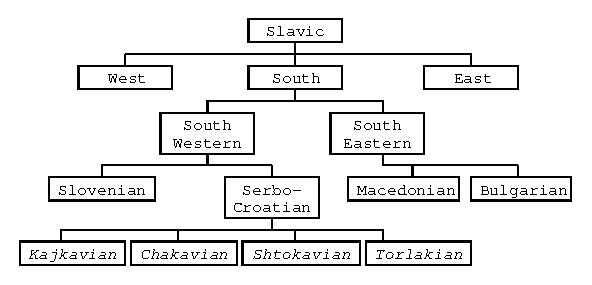
\includegraphics[width=0.5\textwidth]{images/chart.eps}
\caption{A traditional division of the South-Slavic languages. All four standard varieties
     of Serbo-Croatian (Bosnian, Croatian, Montenegrin, and Serbian) are based on the 
     štokavian dialect.}
\end{figure}

\begin{table*}
\centering
\begin{tabular}{lcccc}
  \hline
              &  \textbf{Bosnian} & \textbf{Croatian} & \textbf{Montenegrin} & \textbf{Serbian}\\
  \hline
 \textbf{Čakavian}  & - & -i-,-e-,-je- & - & -  \\
 \textbf{Kajkavian}  & - & -e-,-ie-,-ei,-i- & - & -  \\
 \textbf{Štokavian}  & -ije-,-je- & -ije-,-je-,-i- & -ije-,-je- & -e-,-ije-,-je-  \\
 \textbf{Torlakian}  & - & - & - & -e-  \\
\hline
\end{tabular}
\caption{Intersection of Serbo-Croatian languages and dialects. All four standard variants 
  are based on the štokavian dialect, but other dialects are considered to \emph{belong} to a 
  standard. The entries in the table 
  %-ije-, -e-, and -i- 
  correspond to the \emph{yat} reflex.}
\end{table*}

%% \begin{figure}

%% \todo{Venn diagram of Serbo-Croatian, Serbian, Croatian, Bosnian, Montenegrin, 
%% Neo-Štokavian, Čakavian, Kajkavian, Torlakian
%% Ekavian, Ijekavian, Ikavian}

%% \end{figure}

